\documentclass[a4paper]{article}

\usepackage[pdftex]{graphicx} % Required for including pictures
\usepackage[serbianc]{babel}
\usepackage[pdftex,linkcolor=black,pdfborder={0 0 0}]{hyperref} % Format links for pdf
\usepackage{calc} % To reset the counter in the document after title page
\usepackage{enumitem} % Includes lists
\linespread{1.2} % Set linespace
\usepackage[a4paper, lmargin=0.1\paperwidth, rmargin=0.1\paperwidth, tmargin=0.1\paperheight, bmargin=0.1\paperheight]{geometry} %margins
\edef\restoreparindent{\parindent=\the\parindent\relax}
\usepackage{parskip}
\restoreparindent
\usepackage{float}
\usepackage[bottom]{footmisc}
\usepackage{listings}

\hypersetup{unicode}
\makeindex

\usepackage{url}

\usepackage[all]{nowidow} % Tries to remove widows
%\usepackage[protrusion=true,expansion=true]{microtype} % Improves typography, load after fontpackage is selected

\title{Интегрисани информациони систем за издавање диплома и конкурс за упис на високошколске установе еФакултет}
\author{Борисав Живановић}

\begin{document}

\maketitle

\large

\section*{Сажетак}

У раду је описан интегрисани информациони систем за издавање диплома и конкурс за упис на високошколске установе еФакултет.
Применом овог решења омогућено је централизовано издавње и праћење издатих диплома акредитованих вискошколских установа.
Конкурс за упис се ослања на централизоване регистре диплома средњих школа и високошколских установа.

\section*{Кључне речи}

информациони систем, високо образовање, факултет, диплома, еУправа

\section*{Увод}

Конкурисање за упис на високошколске установе захтева подношење дипломе претходног нивоа образовања.
Такође, конкурисање за посао често захтева доказ о завршеном степену школовања за одређену професију.
Традиционални приступ подношења папирних диплома је подложан злоупотреби, како због подношења фалсификованих диплома,
тако и због немогућности праћења издатих диплома. Аутоматизовано и централизовано праћење података о издатим дипломама
омогућава већу транспарентност у односу на традиционални приступ и олакшава праћење издатих диплома.

\section*{Сродна истраживања}

Већина факултета има информациони систем студентске службе у којем се чувају подаци о издатим дипломама матичног факултета.
На је \autoref{fig:ftn1}, \autoref{fig:ftn2}, \autoref{fig:ftn3} дат приказ изгледа информационог система студентске службе Факултета техичких наука Универзитета у Новом Саду.
Мањи број факултета (попут Факултета техичких наука Универзитета у Новом Саду) имају информациони систем за конкурс, али
као доказ о завршеном претходном нивоу школовања се подносе скениране папирне дипломе. Такав приступ захтева ручну проверу
исправности диплома и повећава вероватноћу за грешком (погрешно унет просек, прихватање фалсификоване дипломе).

\begin{figure}[H]
    \centering
    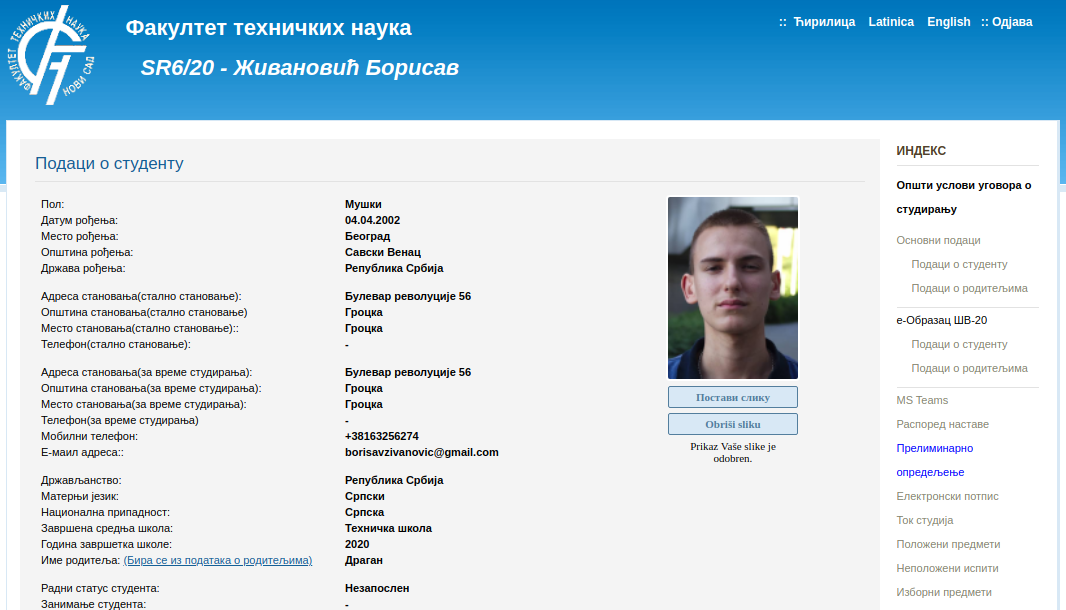
\includegraphics[width=0.5\textwidth,keepaspectratio]{images/ftn1.png}
    \caption{Информације о студенту (студентска служба ФТН УНС)}
    \label{fig:ftn1}
\end{figure}

\begin{figure}[H]
    \centering
    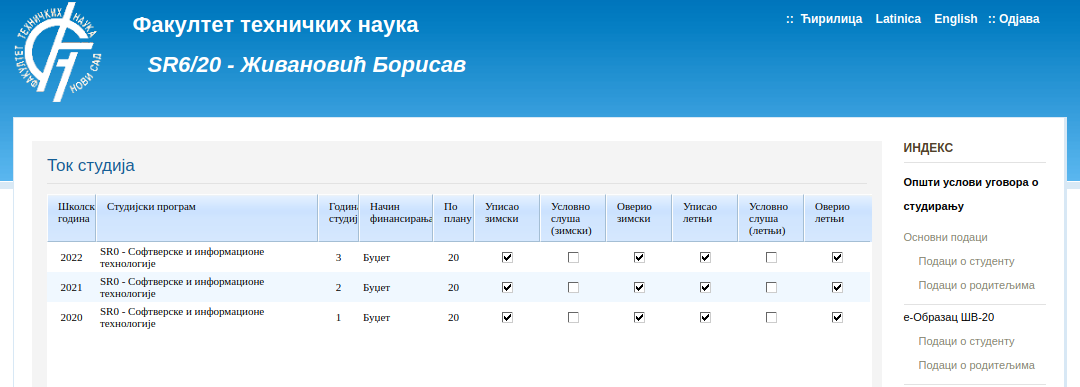
\includegraphics[width=0.5\textwidth,keepaspectratio]{images/ftn2.png}
    \caption{Информације о току студија (студентска служба ФТН УНС)}
    \label{fig:ftn3}
\end{figure}

\begin{figure}[H]
    \centering
    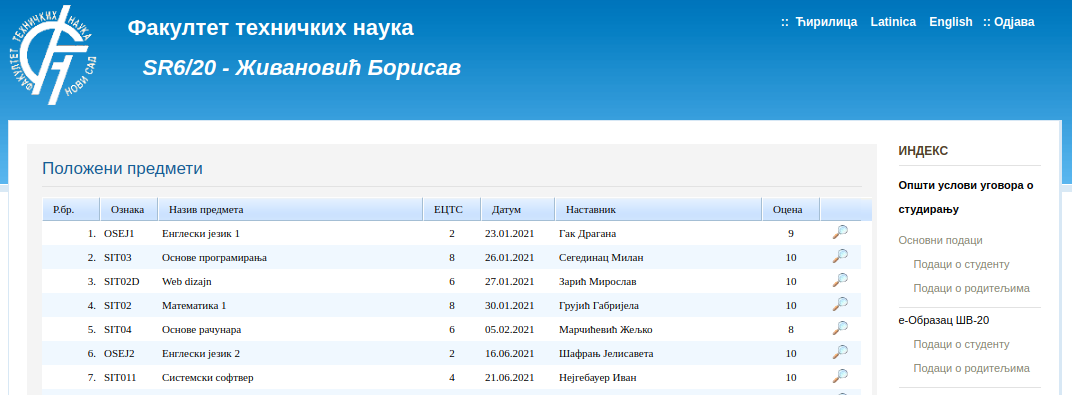
\includegraphics[width=0.5\textwidth,keepaspectratio]{images/ftn3.png}
    \caption{Положени испити (студентска служба ФТН УНС)}
    \label{fig:ftn3}
\end{figure}

\section*{Коришћене технологије}

За имплементацију клијентске апликације коришћен је програмски језик TypeScript\cite{typescript} и окружење (енгл. framework) Angular\cite{angular}.
За имплементацију клијентске апликације коришћен је програмски језик Java\cite{java} и окружење Spring\cite{spring}, уз библиотеку за објектно-релационо мапирање Hibernate\cite{hibernate}.
За ауторизацију је коришћен централизовани SSO (Single Sign On)\footnote{SSO омогућава употребу истих креденцијала за пријаву на више сервиса. Креденцијали се складиште на SSO серверу. Представља концепт, а не стандард који диктира начин имплементације. За више детаља погледати: \href{https://www.onelogin.com/learn/how-single-sign-on-works}{How Does Single Sign-On Work?}}
сервер еУправе (модификована верзија протокола OAuth 2.0\cite{oauth}).
За складиштење података коришћена је MySQL\cite{mysql} база података.

\section*{Спецификација захтева}

Корисници система су администратор и студент. Администратор расписује конкурс (са одговарајућим квотама) и окончава пријаве,
а потом и конкурс. По окончавању конкурса, систем рангира пријаве по просеку, и пријављени из горњег дела ранг листе
(по квоти) добијају могућност за упис. Администратор уноси податке о завршетку студија. Студент се пријављује по конкурсу, уз диплому из регистра. По изласку резултата, прихвата или одбија упис (уколико је распоређен по квоти за упис). Слика \autoref{fig:use_case_diagram} представља детаљан дијаграм случајева коришћења.

\begin{figure}[H]
    \centering
    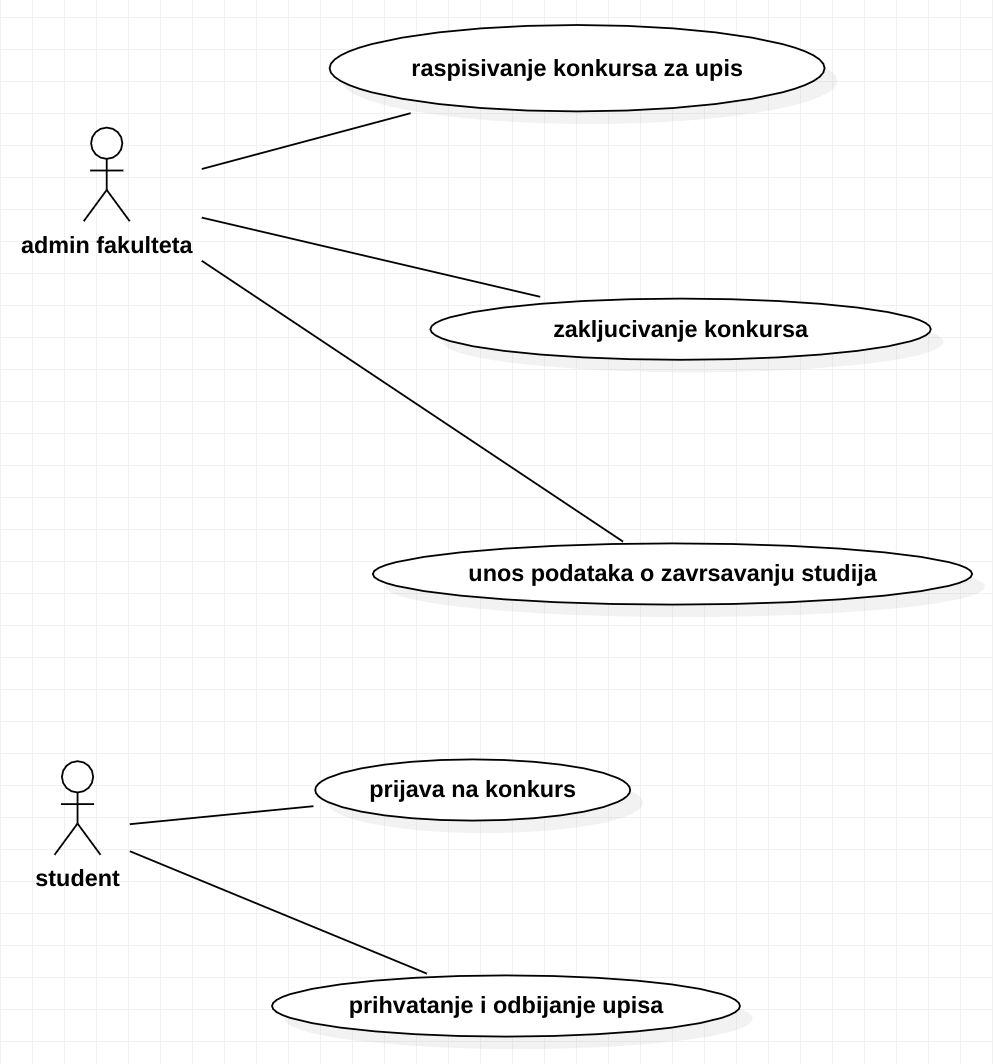
\includegraphics{images/use_case_diagram.png}
    \caption{Дијаграм случајева коришћења}
    \label{fig:use_case_diagram}
\end{figure}

\section*{Спецификација дизајна}

\subsection*{Архитектура система}

Систем је реализован као веб апликација. Клијентска апликација комуницира преко HTTP API-ја са серверском апликацијом. API је
дизајниран у складу са REST архитектонским стилом\cite{rest}. Слика \autoref{fig:app_architecture} приказује архитектуру система.

\begin{figure}[H]
    \centering
    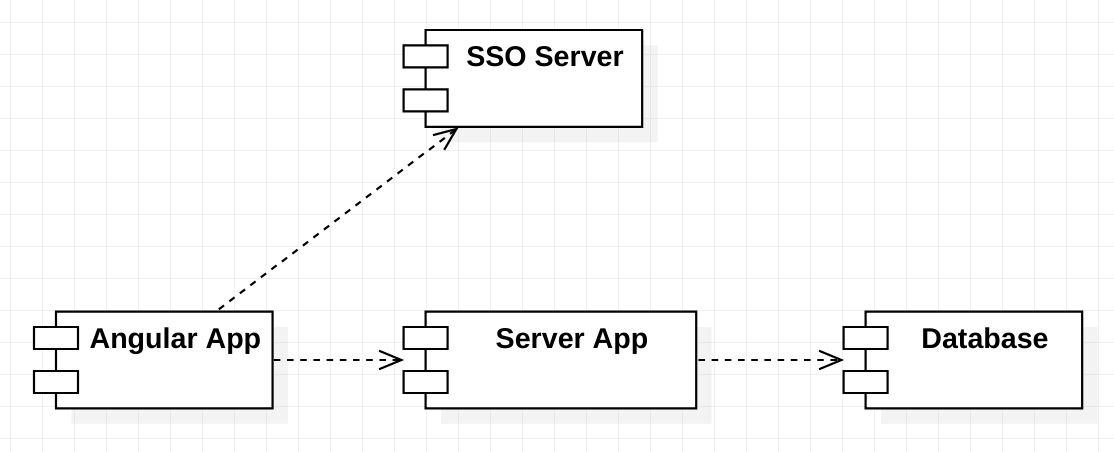
\includegraphics{images/app_architecture.png}
    \caption{Архитектура система}
    \label{fig:app_architecture}
\end{figure}

\subsection*{Модел података}

На слици \autoref{fig:class_diagram} је приказан модел података иницијалне имплементације система. Модел података задовољава трећу нормалну форму, са
изузетком пријава на конкурс, где се у оквиру пријаве чува просек са претходног нивоа образовања.

\begin{figure}[H]
    \centering
    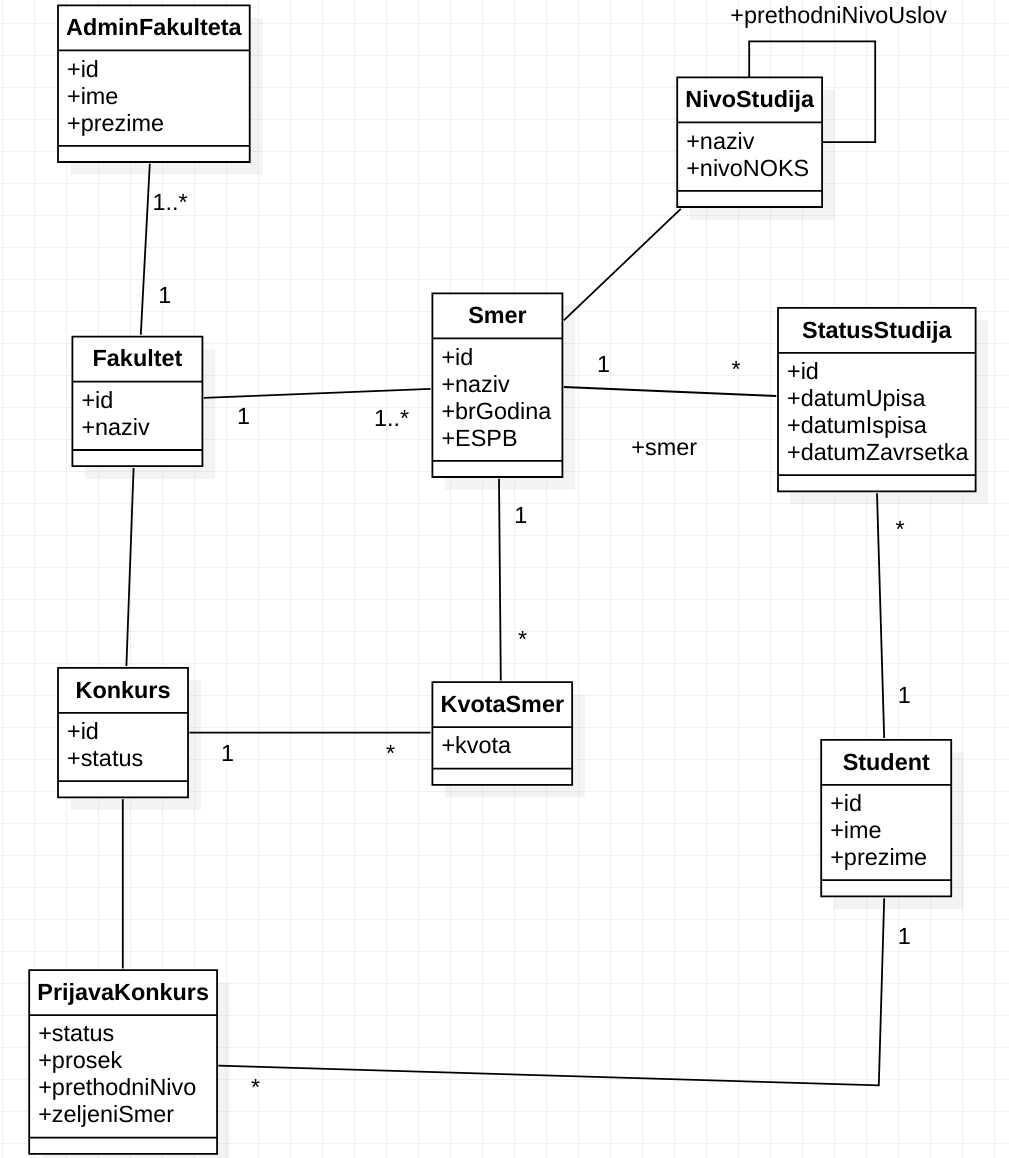
\includegraphics{images/class_diagram.png}
    \caption{Модел података}
    \label{fig:class_diagram}
\end{figure}

Класама Admin и Student представљени су корисници система, а њиховим везама са осталим ентитетима одређена су њихова права приступа. У систему се не чувају лозинке.

Класа PrijavaKonkurs представља учествовање студента на конкурсу кроз све фазе (расписан, затворене пријаве, затворен конкурс).
По затварању конкурса, систем рангира пријаве по просеку и прихваћеним пријавама поставља статус PRIHVACEN.

Класа Studiranje представља период студирања одређеног смера (представљеног класом Smer). Уколико је ниво студија
успешно окончан, садржи датум завршетка и просек. Представља диплому којом је могуће учествовати у конкурсу за упис
на наредни ниво студија.

Класа Konkurs представља један конкурс за упис на факултет. Квота 0 значи да се у датом конкурсу не врши упис студената за дати смер.

\section*{Имплементација}

\subsection*{Клијент}

Клијентска апликација садржи администраторске и студентске функционалности, којима је приступ могућ у зависности од
типа корисника. Тип корисника и привилегије су садржане у токену за ауторизацију. Приступ страницама је контролисан уз guard механизам који прижа Angular.

По потреби, опције су приказане или сакривене као у примеру.

\subsection*{Сервер}

Серверска апликација омогућава приступ систему кроз REST API\cite{rest}. За комуникацију са сервером, неопходан је валидан токен издат од стране еУправа SSO сервера.

Компоненте серверске апликације су приказане на слици \autoref{fig:server_architecture}.

\begin{figure}[H]
    \centering
    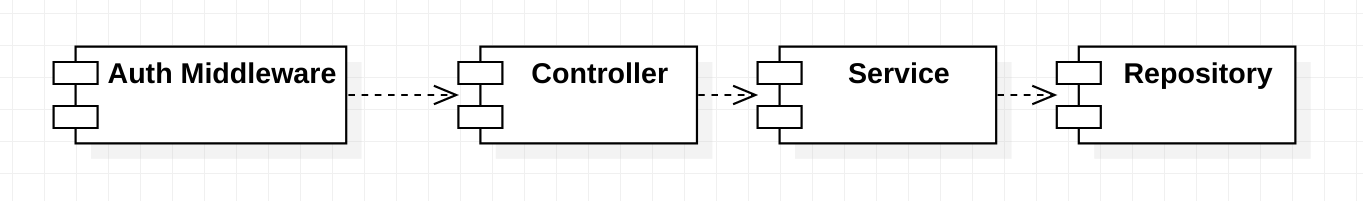
\includegraphics{images/server_architecture.png}
    \caption{Архитектура серверске апликације}
    \label{fig:server_architecture}
\end{figure}

Компонента AuthMiddleware преузима токен из заглавља Authorization из захтева и проверава исправност. Уколико је токен 
исправан, захтев се прослеђује даље у систем. Уколико токен није исправан, захтев се одбија уз грешку 403 Forbidden.

Компонента Controller прослеђује захтев са одговарајућег REST API\cite{rest} на одговарајућу методу сервисног слоја. Садржај
захтева преводи у одговарајуће структуре података програмског језика Java и резултат позива преводи у одговарајући HTTP одговор. Садржи грубу логику за ауторизацију по RBAC\cite{rbac} моделу. Те провере нису довољне, али смањују оптерећење базе података и олакшавају читљивост кода.

\begin{figure}[H]
\begin{lstlisting}[caption={Пример Controller методе},label={lst:controller},captionpos=b]
@GetMapping("/{id}")
public Fakultet getFakultet(@PathVariable long id) {
    return fakultetService.getFakultet(id);
}
\end{lstlisting}
\end{figure}

Компонента Service садржи апликативну логику. Једна сервисна метода одговара једној корисничкој акцији. Садржи комплетне
провере права приступа на нивоу објекта, уз ослонац на ABAC\cite{abac} модел и уз додатне провере апликативне логике
(пример: нису могуће две пријаве истог студента на исти конкурс). У тренутној имплементацији, дата је предност употреби
објектно-релационог мапирања у односу на писање SQL упита због разумљивости кода и брзине имплементације.

\begin{figure}[H]
\begin{lstlisting}[caption={Пример Service методе},label={lst:service},captionpos=b]
public long raspisiKonkurs(long fakultetId, Konkurs konkurs) {
    Fakultet fakultet = fakultetRepository.getById(fakultetId);

    konkurs.setFakultet(fakultet);
    konkurs.setDatumRaspisivanja(LocalDate.now());

    for(KvotaSmer kvotaSmer : konkurs.getKvote()) {
        kvotaSmerRepository.save(kvotaSmer);
    }

    konkursRepository.save(konkurs);

    return konkurs.getId();
}
\end{lstlisting}
\end{figure}

Компонента Repository садржи конкретне упите ка бази података. Једна метода одговара једном упиту. Дата је предност
употреби JPQL у односу на SQL због веће читљивости кода и једноставнијег преласака на други систем за управљање базом података (енгл. Database Management System). Употребом парамтеризованих упита је спречена могућност извођења SQL injection напада
\footnote{SQL injection представља напад у којем нападач злоупотребљава наивни механизам конкатенације стрингова у формирању упита ка бази података.
Иако апликација може да садржи адекватну логику за ауторизацију, њено заобилажење је могуће уколико дозволимо нападачу да утиче на креирање упита.
За више детаља погледати: \href{https://portswigger.net/web-security/sql-injection}{SQL injection}}.

\begin{figure}[H]
\begin{lstlisting}[caption={Пример Repository методе},label={lst:repository},captionpos=b]
@Query("SELECT k FROM Konkurs k WHERE k.fakultet.id = ?1")
List<Konkurs> getKonkursiByFakultetId(long fakultetId);
\end{lstlisting}
\end{figure}

\section*{Демонстрација}

По пријављивању у систем, кориснику је приказан панел који одговара његовој улози (\autoref{fig:admin_panel}, \autoref{fig:student_panel}). 
Администратор има приказ конкурса његове установе (\autoref{fig:admin_konkursi}), као и могућност
расписивања нових конкурса (\autoref{fig:admin_raspisivanje_konkursa}).
Студент има приказ свих тренутно активник конкурса са свих факултета (\autoref{fig:student_konkursi}), као и могућност пријаве на конкурс.

\begin{figure}[H]
    \centering
    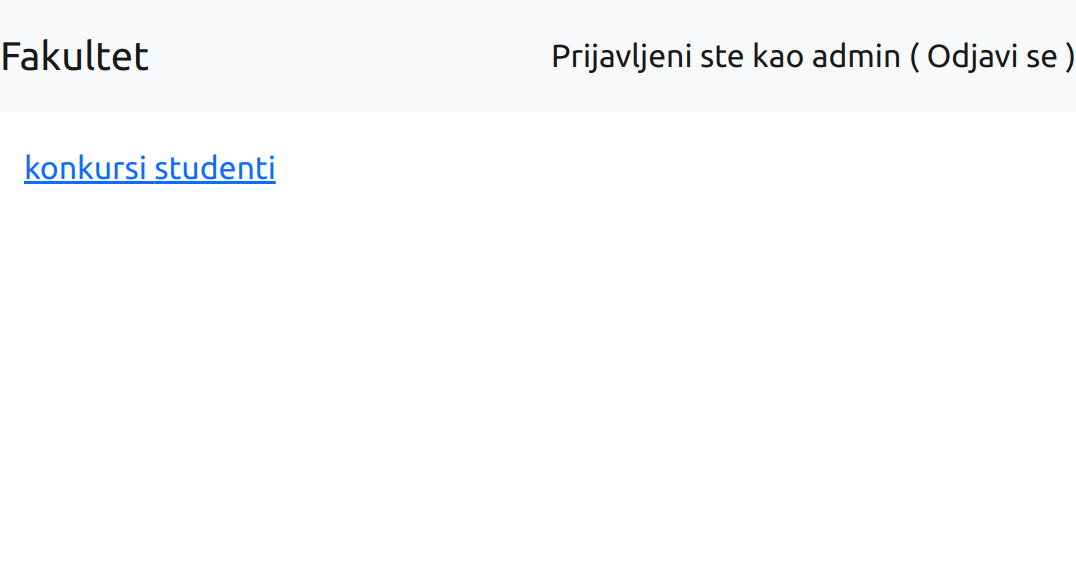
\includegraphics[width=0.5\textwidth,keepaspectratio]{images/admin_panel.png}
    \caption{Администраторски панел}
    \label{fig:admin_panel}
\end{figure}

\begin{figure}[H]
    \centering
    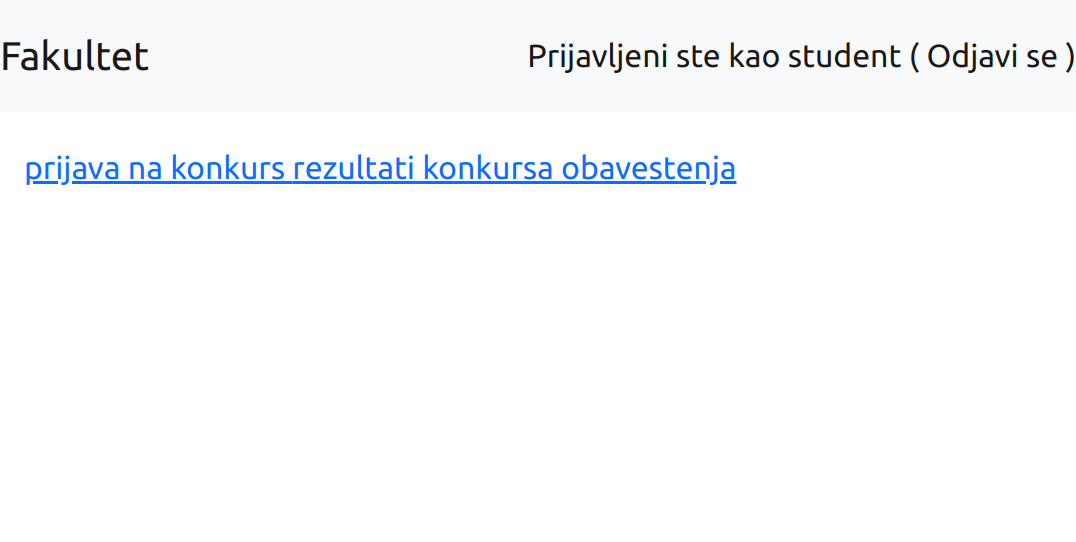
\includegraphics[width=0.5\textwidth,keepaspectratio]{images/student_panel.png}
    \caption{Студентски панел}
    \label{fig:student_panel}
\end{figure}

\begin{figure}[H]
    \centering
    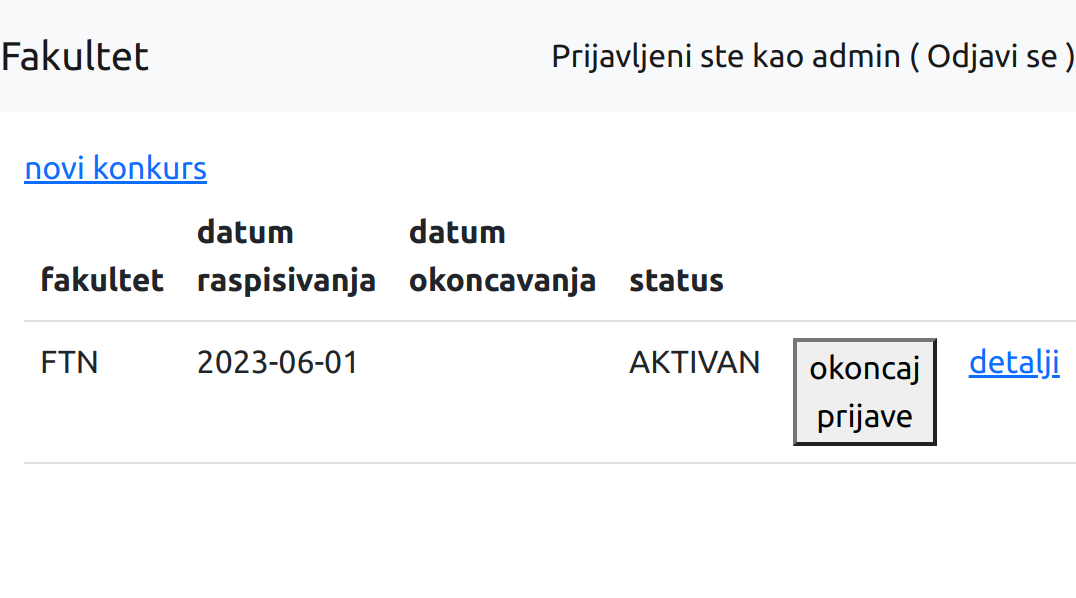
\includegraphics[width=0.5\textwidth,keepaspectratio]{images/admin_konkursi.png}
    \caption{Администраторска страница са конкурсима}
    \label{fig:admin_konkursi}
\end{figure}

\begin{figure}[H]
    \centering
    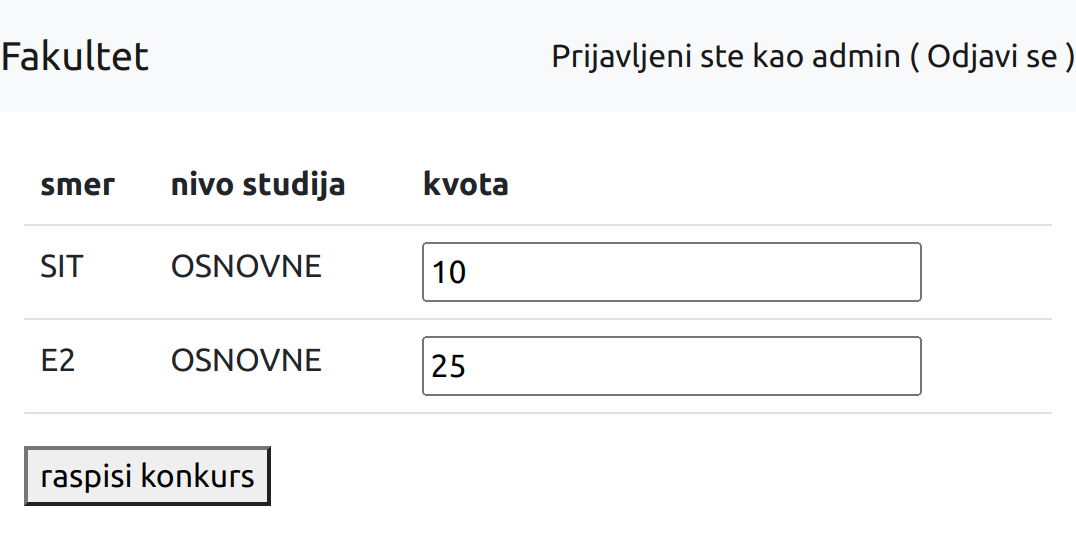
\includegraphics[width=0.5\textwidth,keepaspectratio]{images/admin_raspisivanje_konkursa.png}
    \caption{Расписивање конкурса}
    \label{fig:admin_raspisivanje_konkursa}
\end{figure}

\begin{figure}[H]
    \centering
    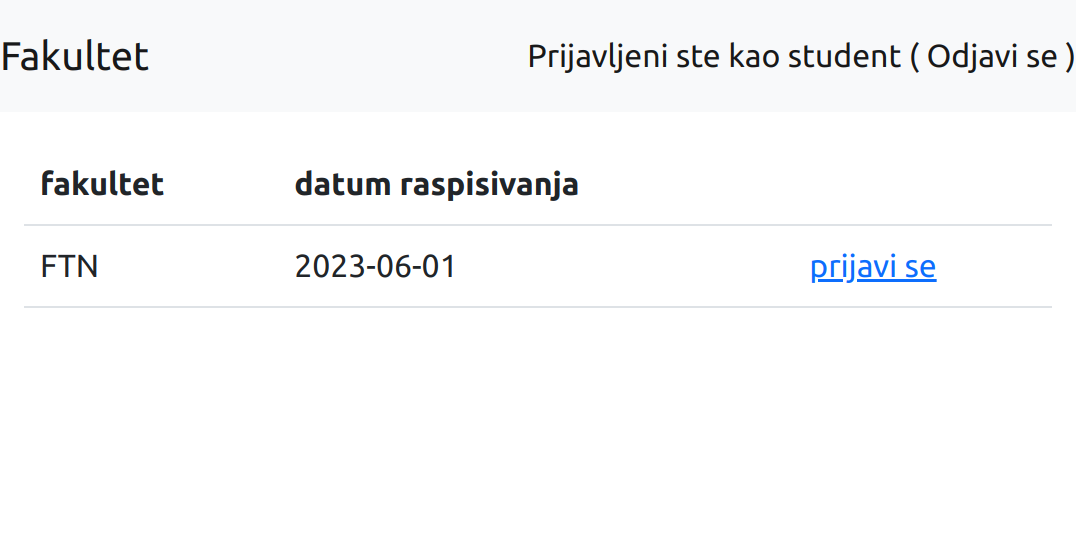
\includegraphics[width=0.5\textwidth,keepaspectratio]{images/student_konkursi.png}
    \caption{Приказ свих активних конкурса}
    \label{fig:student_konkursi}
\end{figure}

\section*{Закључак}

У раду је описан интегрисани информациони систем за издавање диплома и конкурс за упис на високошколске установе еФакултет.
Приказано је како је применом централизованих регистара диплома средњих школа и високошколских установа могуће убразати
конкурс, као и смањити могућност грешки и представљања фалсификованих диплома. У тренутној имплементацији, регистар диплома
и конкурс су обједињени у један систем. У будућности, могуће је раздвајање на две групе система:
централизовани државни регистар диплома и на појединачне системе за конкурс (прилагођене специфичним потребама и
правилима конкурса). Могућ правац развоја би био омогућавање јавног приступа подацима о завршеним степенима образовања
државних функционера, службеника као и осталих лица од важности (лекара, наставника). За имплементацију такве функционалности
би било потребно доношење додатних законских оквира.

\bibliographystyle{plainurl}
\bibliography{refs}

\end{document}
